% Options for packages loaded elsewhere
\PassOptionsToPackage{unicode}{hyperref}
\PassOptionsToPackage{hyphens}{url}
%
\documentclass[
]{article}
\usepackage{amsmath,amssymb}
\usepackage{lmodern}
\usepackage{iftex}
\ifPDFTeX
  \usepackage[T1]{fontenc}
  \usepackage[utf8]{inputenc}
  \usepackage{textcomp} % provide euro and other symbols
\else % if luatex or xetex
  \usepackage{unicode-math}
  \defaultfontfeatures{Scale=MatchLowercase}
  \defaultfontfeatures[\rmfamily]{Ligatures=TeX,Scale=1}
\fi
% Use upquote if available, for straight quotes in verbatim environments
\IfFileExists{upquote.sty}{\usepackage{upquote}}{}
\IfFileExists{microtype.sty}{% use microtype if available
  \usepackage[]{microtype}
  \UseMicrotypeSet[protrusion]{basicmath} % disable protrusion for tt fonts
}{}
\makeatletter
\@ifundefined{KOMAClassName}{% if non-KOMA class
  \IfFileExists{parskip.sty}{%
    \usepackage{parskip}
  }{% else
    \setlength{\parindent}{0pt}
    \setlength{\parskip}{6pt plus 2pt minus 1pt}}
}{% if KOMA class
  \KOMAoptions{parskip=half}}
\makeatother
\usepackage{xcolor}
\usepackage[margin=1in]{geometry}
\usepackage{longtable,booktabs,array}
\usepackage{calc} % for calculating minipage widths
% Correct order of tables after \paragraph or \subparagraph
\usepackage{etoolbox}
\makeatletter
\patchcmd\longtable{\par}{\if@noskipsec\mbox{}\fi\par}{}{}
\makeatother
% Allow footnotes in longtable head/foot
\IfFileExists{footnotehyper.sty}{\usepackage{footnotehyper}}{\usepackage{footnote}}
\makesavenoteenv{longtable}
\usepackage{graphicx}
\makeatletter
\def\maxwidth{\ifdim\Gin@nat@width>\linewidth\linewidth\else\Gin@nat@width\fi}
\def\maxheight{\ifdim\Gin@nat@height>\textheight\textheight\else\Gin@nat@height\fi}
\makeatother
% Scale images if necessary, so that they will not overflow the page
% margins by default, and it is still possible to overwrite the defaults
% using explicit options in \includegraphics[width, height, ...]{}
\setkeys{Gin}{width=\maxwidth,height=\maxheight,keepaspectratio}
% Set default figure placement to htbp
\makeatletter
\def\fps@figure{htbp}
\makeatother
\setlength{\emergencystretch}{3em} % prevent overfull lines
\providecommand{\tightlist}{%
  \setlength{\itemsep}{0pt}\setlength{\parskip}{0pt}}
\setcounter{secnumdepth}{-\maxdimen} % remove section numbering
\usepackage{booktabs}
\usepackage{siunitx}

  \newcolumntype{d}{S[
    input-open-uncertainty=,
    input-close-uncertainty=,
    parse-numbers = false,
    table-align-text-pre=false,
    table-align-text-post=false
  ]}
  
\usepackage{longtable}
\usepackage{array}
\usepackage{multirow}
\usepackage{wrapfig}
\usepackage{float}
\usepackage{colortbl}
\usepackage{pdflscape}
\usepackage{tabu}
\usepackage{threeparttable}
\usepackage{threeparttablex}
\usepackage[normalem]{ulem}
\usepackage{makecell}
\usepackage{xcolor}
\ifLuaTeX
  \usepackage{selnolig}  % disable illegal ligatures
\fi
\IfFileExists{bookmark.sty}{\usepackage{bookmark}}{\usepackage{hyperref}}
\IfFileExists{xurl.sty}{\usepackage{xurl}}{} % add URL line breaks if available
\urlstyle{same} % disable monospaced font for URLs
\hypersetup{
  pdftitle={Characterizing the relationship between the religious affiliation and incidences of Covid-19 at U.S. universities.},
  pdfauthor={Daniel de Castro and Laura Appleby},
  hidelinks,
  pdfcreator={LaTeX via pandoc}}

\title{Characterizing the relationship between the religious affiliation
and incidences of Covid-19 at U.S. universities.}
\author{Daniel de Castro and Laura Appleby}
\date{December 14, 2022}

\begin{document}
\maketitle

\hypertarget{introduction}{%
\section{Introduction}\label{introduction}}

Although the Covid-19 pandemic may feel like a thing of the past, there
is still much research to do in order to understand its nascence,
spread, and lasting health effects. Indeed, we, as a society, must be
prepared to handle the next highly-transmissible pathogen that may
arise. As university students whose first two years in school were far
from normal on account of the Covid-19 pandemic --- whose lives were
dominated by case counts and triweekly testing --- we are interested in
exploring the development of the pandemic at colleges and universities
across the United States. In particular, we are interested in the
differences in how different academic institutions were affected by the
pandemic.

It has been well established that, at least in the United States,
responses to the Covid-19 pandemic were tightly bound to political and
ideological questions, the responses to which differ across the
administrations of the wide range of universities in this country. In
this paper, we will explore the differences in the impact of the
pandemic between institutions with religious affiliations and those
without religious affiliations. We will attempt to characterize the
relationship between case counts during the fall and spring semesters of
the 2020-21 academic year --- the academic year in which responses to
the pandemic were perhaps most varied across universities --- and
whether a university has a religious affiliation. We not only hope to
answer the question of whether religious affiliation has a statistically
significant relationship with case counts during the 2020-21 academic
year --- we also hope to discover the other characteristics of
universities may have an effect on this relationship. To do so, we will
employ a range of statistical inference procedures, from group testing
to hierarchical multilevel models.

\hypertarget{description-of-data-and-source}{%
\section{Description of data and
source}\label{description-of-data-and-source}}

Our data for this project comes from three sources:

\begin{enumerate}
\def\labelenumi{\arabic{enumi}.}
\item
  \href{https://github.com/nytimes/covid-19-data/tree/master/colleges}{NYTimes
  Covid-19 Data}. This data set is publicly available on GitHub and was
  the source for various New York Times maps and visuals in its coverage
  of the pandemic. It includes case counts from July 2020 - May 2021,
  and we have specifically selected cases at Universities. This dataset
  has 1948 entries and includes 2020 cases, 2021 cases, University IPEDS
  ID, University Name, State, etc.
\item
  \href{https://nces.ed.gov/ipeds/use-the-data}{IPEDS Data Center}. This
  is a publicly available data set on colleges and universities across
  the globe. It has many possible variables including demographics,
  admission rates, religious affiliation, etc. The IPEDS data center
  allowed us to select which variables to include in our data set. The
  smallest subset of universities that included all from the NYTimes
  database (by IPEDS ID) was 6125 rows, with all U.S. universities.
\item
  \href{https://data.cdc.gov/Policy-Surveillance/U-S-State-and-Territorial-Public-Mask-Mandates-Fro/tzyy-aayg}{Centers
  for Disease Control}. This publicly available data set tracks mask
  mandates in each state from April 8, 2020, to August 15, 2021.
\item
  The presidential elections data from STAT 139 Problem Set 4. Of this
  data set, we will be particularly focused on the \texttt{gap20repub}
  predictor, which we will use to help characterize the political
  climate of the state in which each institution is located.
\end{enumerate}

After removing universities that were missing lots of data in the pull
from the IPEDS data center, we were left with \(n = 1,705\)
observations.

\hypertarget{data-cleaning-procedures}{%
\section{Data Cleaning Procedures}\label{data-cleaning-procedures}}

Our first step in cleaning the data is to read our data from CSV files
into R data frames. The \texttt{colleges} data frame stores the NYT data
on Covid cases at universities, while the \texttt{ipeds} data frame
stores the data will most of our predictor variables (university
characteristics) taken from IPEDS. We then rename most of the columns in
\texttt{ipeds} to make them shorter and easier to work with.

Next, we merge the \texttt{colleges} and \texttt{ipeds} data frames on
the \texttt{ipeds\_id} column and remove institutions with no IPEDS
data. We then create the \texttt{religious} and \texttt{private}
columns, which are simply indicators for whether an institution has any
religious affiliation, whether it has a catholic affiliation, and
whether it is a private university. Finally, we drop any unnecessary or
redundant columns from the data frame.

We then look to add a column to the data frame that addresses the extent
to which mask mandates were present in the state in which each
institution is located. We read out the mask mandates data from the CDC
into a data frame from the CSV file, treat the appropriate columns as
factors, and convert \texttt{date} into R's \texttt{Date} type.

The next step is to create a new simpler data frame to merge with the
product of the last manipulations. This data frame contains only two
columns: One with the name of each state, and the other with the number
of days between July 1, 2020, and May 26, 2021, during which face masks
were required in public in that state. We then merge this data frame
with our previous data frame to create \texttt{full.cases}, and create a
column \texttt{total.cases} in \texttt{full.cases} that sums the
\texttt{cases} and \texttt{cases\_2021} columns.

Finally, we read the presidential election data from Problem Set 4 into
a data frame, create a two-column data frame with the columns
\texttt{state} and \texttt{gap20repub}, and merge this data frame with
our data frame of observations on the \texttt{state} variable.

\hypertarget{description-of-variables}{%
\section{Description of variables}\label{description-of-variables}}

After performing the data cleaning procedures outlined above, we are
left with the following predictors:

\begin{itemize}
\item
  \textbf{ipeds\_id} This is the IPEDS id, specific to each institution
  and a commonly used identifier for Universities, created by IPEDS.
\item
  \textbf{institution.name} This is the institution name, as filed by
  each University with IPEDS.
\item
  \textbf{state} The state the university is in. This variable has state
  titles, not abbreviations or codes.
\item
  \textbf{private} ``A classification of whether an institution is
  operated by publicly elected or appointed officials or by privately
  elected or appointed officials and derives its major source of funds
  from private sources'' {[}IPEDS{]}. This is simplified to an
  indicator: ``Yes'' for private, ``No'' for a public school.
\item
  \textbf{religious} Indicator with ``Yes'' if the institution is
  religious, ``No'' if not.
\item
  \textbf{tuition} ``Published tuition and fees, 2020-21 for academic
  year reporters only'' {[}IPEDS{]}.
\item
  \textbf{total.headcount} ``12-month unduplicated headcount: 2020-21''
  {[}IPEDS{]}.
\end{itemize}

We elected to include the following demographic information to account
for established inequalities in wealth and access to healthcare in the
United States.

\begin{itemize}
\item
  \textbf{percent.american.native} ``Percent of 12-month unduplicated
  headcount that are American Indian or Alaska Native'' {[}IPEDS{]}.
\item
  \textbf{percent.asian} ``Percent of 12-month unduplicated headcount
  that are Asian'' {[}IPEDS{]}.
\item
  \textbf{percent.black} ``Percent of 12-month unduplicated headcount
  that are Black'' {[}IPEDS{]}.
\item
  \textbf{percent.hispanic.latino} ``Percent of 12-month unduplicated
  headcount that are Hispanic or Latino'' {[}IPEDS{]}.
\item
  \textbf{percent.pacific.islander} ``Percent of 12-month unduplicated
  headcount that are Native Hawaiian or Other Pacific Islander''
  {[}IPEDS{]}.
\item
  \textbf{percent.white} ``Percent of 12-month unduplicated headcount
  that are White'' {[}IPEDS{]}.
\item
  \textbf{percent.two.more.races} ``Percent of 12-month unduplicated
  headcount that are two or more races'' {[}IPEDS{]}.
\item
  \textbf{percent.NA.race} ``Percent of 12-month unduplicated headcount
  that are race/ethnicity unknown'' {[}IPEDS{]}.
\item
  \textbf{percent.women} ``Percent of 12-month unduplicated headcount
  that are women'' {[}IPEDS{]}.
\end{itemize}

The following predictors were included to better characterize each
institution, including the opportunities available to and the general
level of affluence of the student body, as these factors may be related
to access to healthcare or attitudes towards the Covid-19 pandemic.

\begin{itemize}
\item
  \textbf{grad.rate} ``Graduation rate of first-time, full-time degree
  or certificate-seeking students'' {[}IPEDS{]}. Included in our
  analysis to better characterize each institution, its student body,
  and its
\item
  \textbf{percent.fin.aid} ``Percent of full-time first-time
  undergraduates awarded any financial aid'' {[}IPEDS{]}.
\item
  \textbf{percent.student.loan} ``Percent of full-time first-time
  undergraduates awarded student loans'' {[}IPEDS{]}.
\item
  \textbf{occupational.degree} Indicator for if an occupational
  certificate, degree, or other formal award are offered at the
  institution.
\item
  \textbf{hs.equivalent.degree} Indicator for if a highschool-equivelant
  certificate, degree, or other formal award are offered at the
  institution.
\end{itemize}

Other included predictors:

\begin{itemize}
\item
  \textbf{on.campus.housing} Indicator for if on-campus housing is
  offered at the institution.
\item
  \textbf{dorm.capacity} ``The maximum number of students that the
  institution can provide residential facilities for, whether on or off
  campus. (off-campus dormitory space that is reserved by the
  institution)'' {[}IPEDS{]}.
\item
  \textbf{college} See \texttt{institution.name}.
\item
  \textbf{cases}
\item
  \textbf{cases\_2021}
\item
  \textbf{mask.mandated.days}
\item
  \textbf{total.cases}
\item
  \textbf{gap20repub}
\end{itemize}

\hypertarget{group-testing}{%
\section{Group Testing}\label{group-testing}}

To begin our analyses, we will perform a range of group tests to
determine whether the institutions with a religious affiliation had a
higher true average number of Covid cases than religious institutions
without a religious affiliation. In the following analyses, we will test
whether or not the true average number of cases in the fall semester ---
i.e., the case counts for just 2020 in the NYT data set, \texttt{cases}
--- were different for these two groups of institutions, as well as
whether the true average number of cases for the entire academic year
--- see the description of \texttt{total.cases} --- different for the
two groups of institutions. We will perform both sets of analyses,
because they are so fast and easy to perform and interpret. Later, as we
fit linear models to perform more complicated statistical inference
procedures with respect to our data set, we will demonstrate why a focus
will be placed on case counts from the fall semester only (see
``Determining whether data from 2020 or 2020 and 2021 should be used'').

\hypertarget{checking-the-assumptions-for-t-based-methods}{%
\subsection{\texorpdfstring{Checking the assumptions for \(t\)-based
methods}{Checking the assumptions for t-based methods}}\label{checking-the-assumptions-for-t-based-methods}}

We begin with the most commonly used test for a difference in means: the
Student-\(t\) test. Of course, before we can perform this test, we must
make sure that its underlying assumptions are reasonable. Because we
have no reason to assume that the variances in the observations between
both groups --- religiously affiliated and not religiously affiliated
universities --- are the same, we will use the unpooled \(t\)-test. For
unpooled \(t\)-based test for a difference in sample means, there are
three assumptions:

\begin{enumerate}
\def\labelenumi{\arabic{enumi})}
\item
  \textbf{Observations are independent.} We claim that this observation
  is reasonable. Even though the geographic proximity of universities
  might have caused there to be some correlation between case counts at
  these different schools, we claim that since universities are somewhat
  insular communities --- students tend to stay within their own social
  sphere of their university --- this is not a major concern. Overall,
  with such a rich data set, in which a wide and diverse range of
  characteristics are expressed across all 1,705 observations, this
  assumption of independence of observations seems reasonable.
\item
  \textbf{Groups are independent of one another.} There is no reason to
  suggest that the two groups in question --- religious institutions and
  non-religious institutions --- are not independent from one another.
  Above, we justified that all of the observations in our data set are
  sufficiently independent from one another --- if this is true, then it
  is reasonable to assume that these two groups of institutions are
  independent of one another.
\item
  \textbf{Observations are normally distributed.} As is shown in the
  plot below (left), both of the response variables in question are
  \emph{not} normally distributed; after log-transforming these
  responses, however, we see that their distributions are symmetrical
  enough to satisfy this assumption. Of course, we do not need to seek
  perfect normality with respect to these distributions, since
  \(t\)-based statistical inference procedures are robust to this
  assumption (as was demonstrated in Question 5 in Problem Set 3).
\end{enumerate}

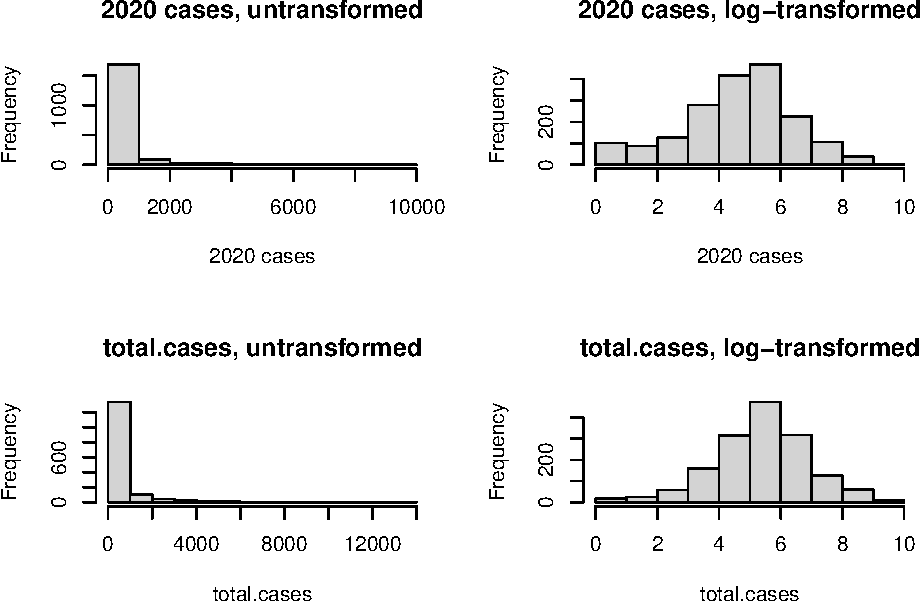
\includegraphics{final_files/figure-latex/unnamed-chunk-8-1.pdf}

The Normal Q-Q Plots below corroborate the conclusion that this
assumption is reasonable. In each plot, the data for the most part
follows the line that we would expect if it were perfectly normally
distributed; although, since the data sits below the line at both the
positive and negative extremes of the graph, the left tail is a bit
fatter and the right tail a bit skinnier than the perfectly normal
distribution in each of these sample distributions.

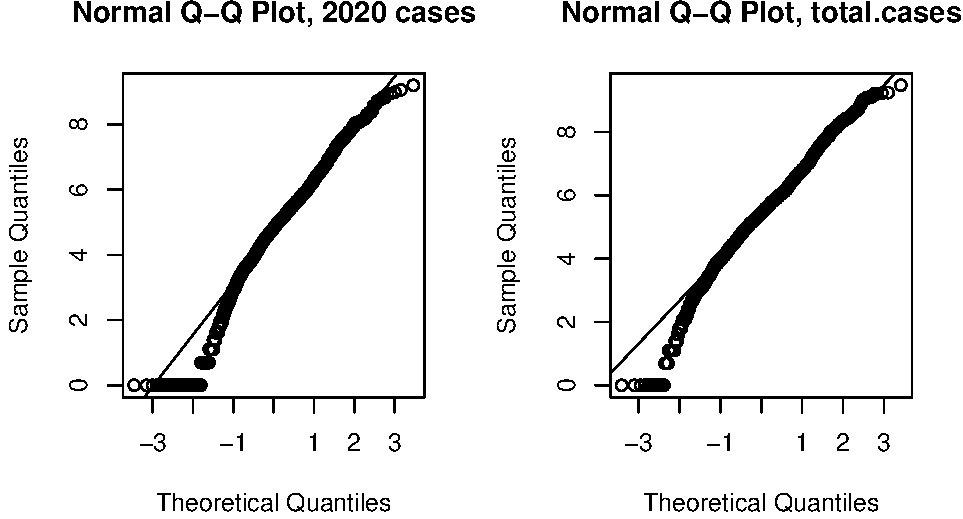
\includegraphics{final_files/figure-latex/unnamed-chunk-9-1.pdf}

\hypertarget{student-t-tests}{%
\subsection{\texorpdfstring{Student-\(t\)
Tests}{Student-t Tests}}\label{student-t-tests}}

Now that we have shown the assumptions of Student-\(t\) tests to be
reasonable, we can proceed to perform the tests themselves. We perform
two two-sided \(t\)-tests for a difference in means. In each case, the
null hypothesis is that the true mean case counts in the two groups ---
religiously affiliated and non-religiously affiliated institutions ---
are equal over the given time period, and the alternative is that they
are not equal. As in the rest of the paper, we will use the standard
confidence level of \(\alpha = 0.05\), for the sake of convenience and
conformity with the wider statistics community. Below are the results
from these tests.

\begin{longtable}[]{@{}lrrr@{}}
\toprule()
sample & test.statistic & df & p.value \\
\midrule()
\endhead
2020 only & 1.379947 & 969.4587 & 0.1679212 \\
entire year & -0.564321 & 885.7181 & 0.5726786 \\
\bottomrule()
\end{longtable}

In both tests, we see that our p-value is greater than the significance
level of 0.05; we thus fail to reject the null hypothesis in both cases
--- we do not have statistically significant evidence to suggest that
the true mean case counts, both for the fall semester and for the entire
year, are different between the religiously affiliated and
non-religiously affiliated institutions. Note that the degrees of
freedom --- which are not integers owing to R's use of the Welch
approximation --- are different for the two tests. This is because the
test using the \texttt{total.cases} data has fewer observations, since
some schools in our sample did not report case counts for the spring
semester. This issue is tackled in greater detail below (see
``Determining whether data from 2020 or 2020 and 2021 should be used'').

\hypertarget{non-parametric-testing-wilcox-rank-sum-test}{%
\subsection{Non-Parametric Testing --- Wilcox Rank Sum
Test}\label{non-parametric-testing-wilcox-rank-sum-test}}

We will also perform the non-parametric Wilcox Rank Sum Test to
determine whether the case counts are different between religiously
affiliated and non-religiously affiliated schools. The strength of this
non-parametric test lies in the fact that it does not rely on an
assumption on the distribution of the data-generating process of the
sample. Thus, though we are confident in having shown above that the
distributions of the log-transformed responses are sufficiently
approximately normal, for the sake of completeness, we will perform this
non-parametric test, and see if it leads us to the same conclusions.

Again, we will perform the Wilcox Rank Sum Test on data from just the
fall semester and on data from the entire academic year. For the
following two tests, the null hypothesis is that the true average
quantiles within the two groups --- when the data from both groups are
ranked together --- are the same, while the alternative hypothesis is
that there is an association between group status and the average
quantile of the observations in the entire population.

\begin{longtable}[]{@{}lrr@{}}
\toprule()
sample & test.statistic & p.value \\
\midrule()
\endhead
2020 only & 320824.0 & 0.2990076 \\
entire year & 225800.5 & 0.7547593 \\
\bottomrule()
\end{longtable}

As the results above show, neither test was statistically significant at
the 0.05 confidence level; we thus again fail to reject the null
hypothesis, concluding that there is no statistically significant
evidence to suggest that the there is an association between religious
affiliation and average quantile of case counts in either sample.

\hypertarget{basic-linear-regression-models}{%
\section{Basic Linear Regression
Models}\label{basic-linear-regression-models}}

Of course, group tests are limited in that they do not take into account
potential confounding variables that might reveal the significance of an
institution's having a religious affiliation. To take into account the
effects of these potential confounding variables --- which we have
already identified at length, as evidenced by the extensive list of
predictors we compiled before beginning our analyses --- we will fit
linear models. We will then use these linear models to perform
statistical inference on the coefficient of the \texttt{religious}
predictor, determining whether there is a statistically significant
relationship between an institution's religious affiliation and the
number of cases that it recorded.

\hypertarget{checking-the-assumptions-of-linear-regression-models}{%
\subsection{Checking the Assumptions of Linear Regression
Models}\label{checking-the-assumptions-of-linear-regression-models}}

Before we can fit more complicated models, we must first check the
assumptions of linear regression. We begin by checking the assumption of
linearity. To do so, we plotted \texttt{cases} versus all of the
quantitative predictors that we would like to include in our analyses.
We the identified that \texttt{total.headcount},
\texttt{percent.american.native}, \texttt{percent.asian},
\texttt{percent.black}, \texttt{percent.hispanic.latino}, and
\texttt{percent.pacific.islander} would benefit from being
log-transformed; given the left-skewness of its distribution, we also
determined that \texttt{percent.fin.aid} would be best transformed using
the following transformation
\texttt{log(100\ -\ percent.fin.aid\ +\ 1)}. The following plots show
that the distribution of these predictors before and after being
transformed. \emph{In these plots, the y-axis is always log-transformed
cases} (2020); the axis label is not printed in order to save space.

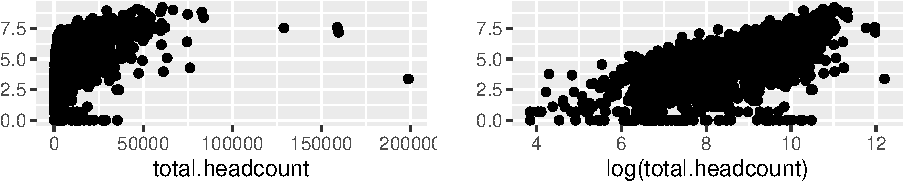
\includegraphics{final_files/figure-latex/unnamed-chunk-12-1.pdf}
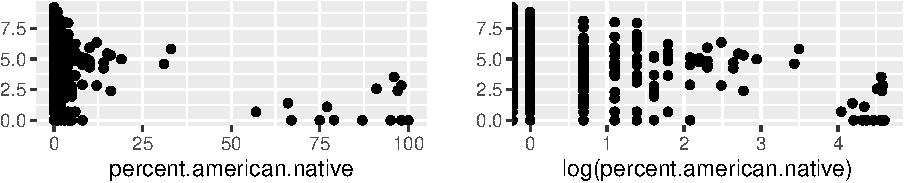
\includegraphics{final_files/figure-latex/unnamed-chunk-12-2.pdf}
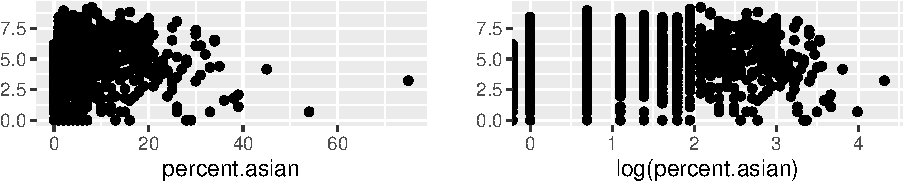
\includegraphics{final_files/figure-latex/unnamed-chunk-12-3.pdf}
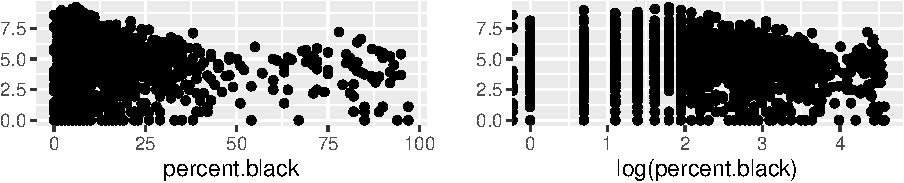
\includegraphics{final_files/figure-latex/unnamed-chunk-12-4.pdf}
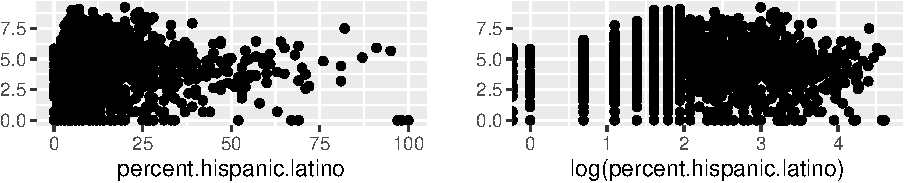
\includegraphics{final_files/figure-latex/unnamed-chunk-12-5.pdf}
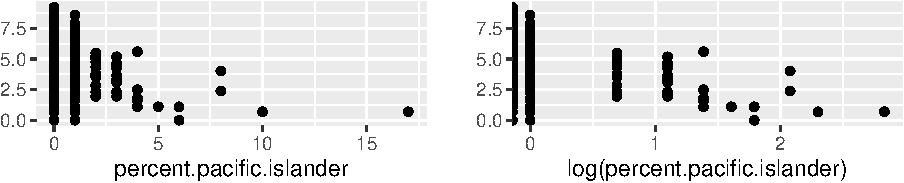
\includegraphics{final_files/figure-latex/unnamed-chunk-12-6.pdf}
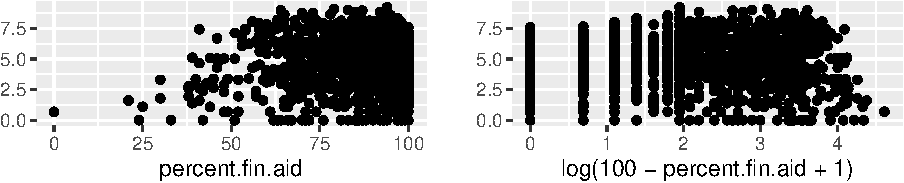
\includegraphics{final_files/figure-latex/unnamed-chunk-12-7.pdf}

We claim that with these transformations, the assumption of linearity is
reasonable.

What remains to be shown is that the assumption of homoskedasticity is
reasonable. In order to check this assumption, we fit basic regression
models for \texttt{cases} and \texttt{total.cases} using all of the
predictors in our predictor set.

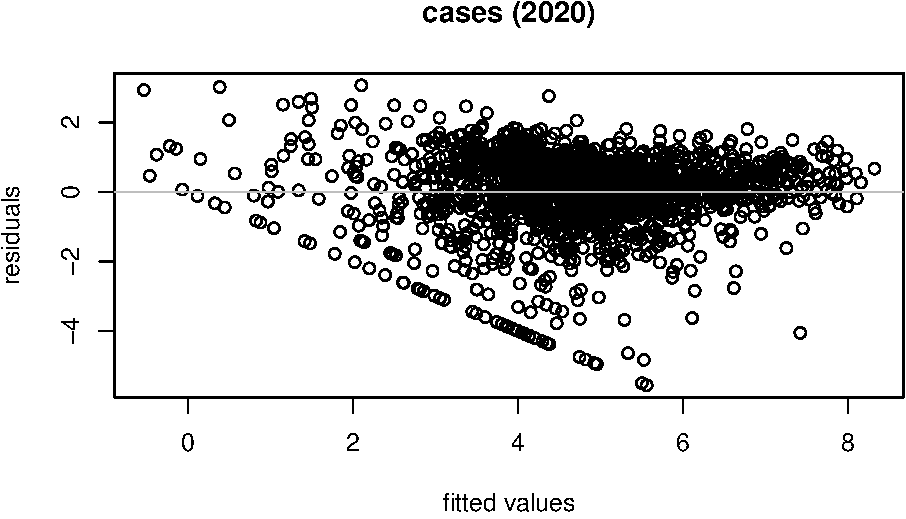
\includegraphics{final_files/figure-latex/unnamed-chunk-13-1.pdf}

As is shown in the plot above, the spread of the residuals is not
constant across the entire range of fitted values --- thus, it is called
into question whether the assumption of homoskedasticity is reasonable
in this case. The behavior of this graph is interesting: Towards the
left extreme of the graph, there appear to be bands of observations
whose positions on this plot form negatively sloped lines. The left-most
line corresponds to all those observations where the case counts are
zero; the second-left-most line corresponds to the observations where
the case counts are one; the next corresponds to the observations where
the case count is two, etc. As one moves closer to the center of the
plot, this pattern disappears, and the plot assumes a form that is much
better suited to linear regression. Thus, this problem arises from the
fact that our response variable is discrete, and from the fact that we
have so many observations with very low case counts. As it stands, we
must be wary of this assumption of homoskedasticity, which might affect
the standard errors that we will use to calculate the statistical
significance of coefficient estimates. Later in the paper, we will
perform a sensitivity analysis using Poisson regression to corroborate
the results we obtain using Gaussian regression.

Below, we recreate the same plot, but for the case counts for the entire
2020-21 academic year.

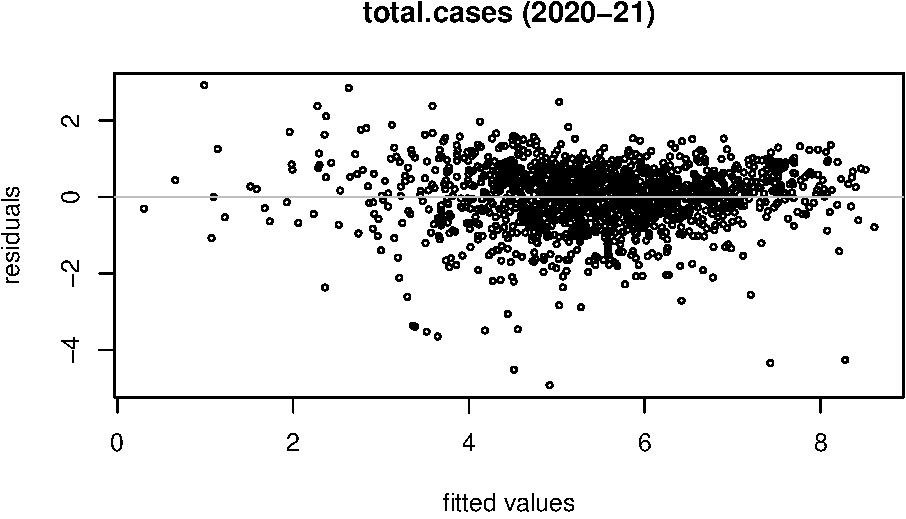
\includegraphics{final_files/figure-latex/unnamed-chunk-14-1.pdf}

In the above plot for the model for \texttt{total.cases}, the spread of
the residuals appears much more consistent across the entire range of
fitted values. If one looks carefully enough, however, they will see
that the same behavior observed in the preceding plot is present in this
one, the difference being that there are fewer schools that reported
very low case counts (0, 1, or 2). This is likely due to the fact that,
with an extra five months of data, our response took on enough different
values to begin to behave more like a continuous variable; in addition,
a not-insignificant number of schools that simply did not report case
data for the spring semester (236 observations).

\hypertarget{determining-whether-data-from-2020-or-2020-and-2021-should-be-used}{%
\subsection{Determining whether data from 2020 or 2020 and 2021 should
be
used}\label{determining-whether-data-from-2020-or-2020-and-2021-should-be-used}}

Naturally, there is a temptation to focus on case data for the entire
academic year (the entire time period during which case data was
collected by the \emph{New York Times}). There is one problem, however:
While the \emph{New York Times} was able to compile case data for all of
the schools in our data set for the fall semester of that year, it was
not able to find data for 236 schools for the spring semester. This is a
nontrivial number of observations given that our data set only consists
of 1,705 different institutions; thus, to determine whether it would be
sound to remove these 236 observations and fit models and perform
statistical inferences on data from the entire academic year, we must
determine whether the two groups of schools in question --- those that
reported data for the entire academic year, and those that did not ---
are sufficiently similar to one another.

The first step is to compare the coefficients of our baseline model
(\texttt{lm6} above) when it is fit to all 1,705 observations, as well
as individually to the two different groups of schools in question. The
coefficient estimates, along with the p-values (not adjusted to be
heteroskedastically consistent) are given in Table 3.

\begin{table}

\caption{\label{tab:unnamed-chunk-15}A comparison of the base model across three different samples.}
\centering
\begin{tabular}[t]{lcccccc}
\toprule
\multicolumn{1}{c}{ } & \multicolumn{2}{c}{all schools} & \multicolumn{2}{c}{\makecell[c]{schools with data\\for both years}} & \multicolumn{2}{c}{\makecell[c]{schools with only\\2020 data}} \\
\cmidrule(l{3pt}r{3pt}){2-3} \cmidrule(l{3pt}r{3pt}){4-5} \cmidrule(l{3pt}r{3pt}){6-7}
  & Est. & p & Est. & p & Est. & p\\
\midrule
(Intercept) & \num{-5.719} & \num{<0.001} & \num{-4.975} & \num{<0.001} & \num{-2.338} & \num{0.109}\\
religiousYes & \num{0.102} & \num{0.252} & \num{0.318} & \num{<0.001} & \num{-0.701} & \num{0.049}\\
tuition & \num{0.00002} & \num{<0.001} & \num{0.00001} & \num{<0.001} & \num{-0.000003} & \num{0.878}\\
log(total.headcount + epsilon) & \num{0.920} & \num{<0.001} & \num{0.915} & \num{<0.001} & \num{0.491} & \num{<0.001}\\
log(percent.american.native + epsilon) & \num{0.013} & \num{0.811} & \num{0.170} & \num{<0.001} & \num{-0.300} & \num{0.072}\\
log(percent.asian + epsilon) & \num{-0.125} & \num{0.026} & \num{-0.225} & \num{<0.001} & \num{-0.0006} & \num{0.998}\\
log(percent.black + epsilon) & \num{0.195} & \num{<0.001} & \num{0.205} & \num{<0.001} & \num{-0.057} & \num{0.716}\\
log(percent.hispanic.latino + epsilon) & \num{0.060} & \num{0.172} & \num{0.075} & \num{0.046} & \num{0.223} & \num{0.110}\\
log(percent.pacific.islander + epsilon) & \num{-0.289} & \num{0.015} & \num{-0.366} & \num{<0.001} & \num{0.118} & \num{0.719}\\
percent.white & \num{0.018} & \num{<0.001} & \num{0.015} & \num{<0.001} & \num{0.014} & \num{0.017}\\
percent.two.more.races & \num{-0.025} & \num{0.026} & \num{-0.015} & \num{0.115} & \num{-0.066} & \num{0.097}\\
percent.women & \num{-0.011} & \num{<0.001} & \num{-0.014} & \num{<0.001} & \num{0.002} & \num{0.784}\\
grad.rate & \num{0.021} & \num{<0.001} & \num{0.020} & \num{<0.001} & \num{0.017} & \num{0.037}\\
log(100 - percent.fin.aid + epsilon) & \num{-0.043} & \num{0.162} & \num{0.024} & \num{0.349} & \num{-0.275} & \num{0.019}\\
on.campus.housingYes & \num{0.823} & \num{<0.001} & \num{0.670} & \num{<0.001} & \num{1.096} & \num{<0.001}\\
gap20repub & \num{0.013} & \num{<0.001} & \num{0.012} & \num{<0.001} & \num{0.028} & \num{<0.001}\\
privateYes & \num{-0.677} & \num{<0.001} & \num{-0.377} & \num{0.003} & \num{-0.475} & \num{0.331}\\
percent.student.loan & \num{0.005} & \num{0.002} & \num{0.007} & \num{<0.001} & \num{-0.0006} & \num{0.923}\\
mask.mandated.days & \num{0.0002} & \num{0.545} & \num{-0.0007} & \num{0.001} & \num{-0.00007} & \num{0.941}\\
occupational.degreeYes & \num{-0.184} & \num{0.017} & \num{-0.011} & \num{0.865} & \num{-0.938} & \num{<0.001}\\
hs.equivalent.degreeYes & \num{0.136} & \num{0.154} & \num{-0.083} & \num{0.287} & \num{0.314} & \num{0.381}\\
\midrule
Num.Obs. & \num{1705} &  & \num{1469} &  & \num{236} & \\
R2 & \num{0.604} &  & \num{0.694} &  & \num{0.408} & \\
R2 Adj. & \num{0.599} &  & \num{0.690} &  & \num{0.353} & \\
Log.Lik. & \num{-2590.545} &  & \num{-1808.194} &  & \num{-424.879} & \\
RMSE & \num{1.11} &  & \num{0.83} &  & \num{1.46} & \\
\bottomrule
\end{tabular}
\end{table}

As we can see, when the sample of the institutions used to fit the model
changes, some of the coefficient estimates change vastly. Take, for
example, the coefficient estimate for \texttt{religionYes}, which can be
interpreted as the natural log of the change in cases that we would
expect if a given school were to have a religious affiliation rather
than not have one. This coefficient estimate is not statistically
significant when all institutions are considered together, is positive
and statistically significant when the institutions that reported data
for the entire academic year are considered, and negative and
statistically significant when the institutions that only reported data
for the fall are considered. In fact, if one were to inspect the table
above, they would notice that the majority of predictors included in
this baseline model experienced changes in their coefficient estimates
and statistical significance as the sample of institutions was changed.

Clearly, then, there are some underlying differences between the schools
that did and the schools that did not report case data for the spring
semester of the 2020-21 academic year. Consider the coefficient estimate
for \texttt{religiousYes}, which is quite different in the two models
fit to data from only one of the two subgroups; this is especially
interesting for our research purposes. Indeed, searching for the
differences between these subgroups in terms of \texttt{religious} and
other predictors might help us to answer the questions about the
association between religious affiliation and reported Covid cases that
are motivating this paper.

First, we investigate the difference in the political leanings of the
states in which these schools were located, as given by
\texttt{gap20repub}. To do so, we perform a \(t\)-test (the assumptions
that allow us to do so have been explored above), with the null
hypothesis being that the true means \texttt{gap20repub} are equal
between the two groups of institutions, and the alternative being that
the true means are different. The result of this test is shown below.

\begin{center}

\begin{tabular}{l|l|r|r|r}
\hline
  & predictor & test.statistic & df & p.value\\
\hline
t & gap20repub & -6.289246 & 445.719 & 0\\
\hline
\end{tabular}
\end{center}

With a p-value that is much smaller than our \(\alpha =0.05\) (again,
because we do not assume equal variances between the groups, the Welch
approximation for degrees of freedom is used), we reject the null
hypothesis, concluding that the true mean \texttt{gap20repub} is
different for the schools that did report case data for 2021 versus
those that did not. As it turns out, the 95\% \(t\)-based confidence
interval for the mean \texttt{gap20repub} for the schools that did
report 2021 case data minus the mean \texttt{gap20repub} for the schools
that did not is (-9.468120, -4.959647) --- thus, we conclude that the
schools that did report 2021 case data are located in states that are
considerably more left-leaning than the schools that did not.

We repeat this sort of analysis for \texttt{total.headcount},
\texttt{tuition}, \texttt{percent.fin.aid}, \texttt{mask.mandated.days},
\texttt{on.campus.housing}, and \texttt{religious}, predictors that we
have chosen based on large differences in the coefficient estimates
produced by the models above when fit to only one of the two subgroups
of institutions. We use a two-sided \(t\)-test for the quantitative
variables and two-sided z-tests for proportions for the
\texttt{categorical} predictors; we also perform the same
transformations as above to make sure that the predictor in question is
approximately normally distributed in each test. The hypotheses are
similar to the \texttt{gap20repub} test, the null being that the true
means/proportions are equal between the two groups, and the alternative
being that they are not equal. As per the results shown below, the tests
for all six of these predictors showed statistically significant
differences between the two groups of universities.

\begin{center}

\begin{tabular}{l|r|r|r}
\hline
predictor & test.statistic & df & p.value\\
\hline
total.headcount & 11.236414 & 419.7951 & 0.0000000\\
\hline
tuition & 3.718410 & 397.6510 & 0.0002293\\
\hline
percent.fin.aid & 0.587267 & 376.8880 & 0.5573761\\
\hline
mask.mandated.days & 8.949245 & 376.7757 & 0.0000000\\
\hline
on.campus.housing & 26.561220 & 1.0000 & 0.0000003\\
\hline
religious & 14.254276 & 1.0000 & 0.0001597\\
\hline
\end{tabular}
\end{center}

The existence of these statistically significant differences between
these two groups of institutions leads us to two distinct conclusions:
Firstly, that we should perform all further analyses on data only from
the fall 2020 semester, and secondly, that we should consider
interaction effects in our model to help better isolate and take into
account these demonstrated differences between these two different
groups of institutions.

\hypertarget{linear-models-with-interaction-effects}{%
\section{Linear Models with Interaction
Effects}\label{linear-models-with-interaction-effects}}

Above we performed several linear regressions with no interactions and
multiple predictors. Our ``base model'' includes all of the predictors
we include in this paper, which are: \texttt{religious},
\texttt{tuition}, \texttt{total.headcount},
\texttt{percent.american.native}, \texttt{percent.asian},
\texttt{percent.black}, \texttt{percent.hispanic.latino},
\texttt{percent.pacific.islander}, \texttt{percent.white},
\texttt{percent.two.more.races}, \texttt{percent.women},
\texttt{grad.rate}, \texttt{percent.fin.aid},
\texttt{on.campus.housing}, \texttt{gap20repub}, \texttt{private},
\texttt{percent.student.loan}, \texttt{mask.mandated.days},
\texttt{occupational.degree} and \texttt{hs.equivelant.degree}. Above we
discuss using 2020 cases, 2021 cases, or the total number of cases,
concluding that we will use only 2020 cases for the remaining models.

We will first look at three linear models with all of the predictors in
this paper: our ``base model,'' an interaction model between the
\texttt{religious} predictor and the others
(\texttt{religiousInteraction}), and a full interaction model
(\texttt{fullInteraction}).

\begin{table}

\caption{\label{tab:unnamed-chunk-18}Significant Predictors from Base Model}
\centering
\begin{tabular}[t]{l|r|r}
\hline
  & coefficients & p.value\\
\hline
tuition & 0.0000174 & 0.0000161\\
\hline
log(total.headcount + epsilon) & 0.9199545 & 0.0000000\\
\hline
log(percent.asian + epsilon) & -0.1251276 & 0.0257048\\
\hline
log(percent.black + epsilon) & 0.1946336 & 0.0000088\\
\hline
log(percent.pacific.islander + epsilon) & -0.2890057 & 0.0146274\\
\hline
percent.white & 0.0178880 & 0.0000000\\
\hline
percent.two.more.races & -0.0254703 & 0.0262692\\
\hline
percent.women & -0.0107628 & 0.0000245\\
\hline
grad.rate & 0.0210106 & 0.0000000\\
\hline
on.campus.housingYes & 0.8225306 & 0.0000000\\
\hline
gap20repub & 0.0127476 & 0.0000000\\
\hline
privateYes & -0.6765733 & 0.0000051\\
\hline
percent.student.loan & 0.0053149 & 0.0017920\\
\hline
occupational.degreeYes & -0.1840886 & 0.0173571\\
\hline
\end{tabular}
\end{table}

Table 4 shows the coefficient estimates from the base model. We see that
there are a lot of statistically significant coefficients on the
predictors (at the \(\alpha=0.05\) level), holding all else constant.
Notably, the coefficient for the \texttt{religious} variable does not
carry statistical significance, with a p-value of .25190, significantly
above \(\alpha = 0.05\). This could be for a number of reasons,
including that 1) religious affiliation (either Yes: Religious or No:
Not Religious) simply has no correlation with 2020 Covid cases or 2) the
\texttt{religious} variable shares predictive power (has some degree of
collinearity) with other predictor variables.

\begin{table}

\caption{\label{tab:unnamed-chunk-19}Significant Predictors from Religious Interaction Model}
\centering
\begin{tabular}[t]{l|r|r}
\hline
  & coefficients & p.value\\
\hline
religiousYes & 3.6653774 & 0.0002896\\
\hline
tuition & 0.0000175 & 0.0007126\\
\hline
log(total.headcount + epsilon) & 0.9491104 & 0.0000000\\
\hline
log(percent.black + epsilon) & 0.2514204 & 0.0000003\\
\hline
log(percent.pacific.islander + epsilon) & -0.3163746 & 0.0229103\\
\hline
percent.white & 0.0190307 & 0.0000000\\
\hline
percent.women & -0.0110546 & 0.0002047\\
\hline
grad.rate & 0.0222312 & 0.0000000\\
\hline
on.campus.housingYes & 0.8374462 & 0.0000000\\
\hline
gap20repub & 0.0131810 & 0.0000000\\
\hline
privateYes & -0.6565577 & 0.0002535\\
\hline
percent.student.loan & 0.0055159 & 0.0041419\\
\hline
religiousYes:log(percent.american.native + epsilon) & -0.4244315 & 0.0100105\\
\hline
religiousYes:log(percent.black + epsilon) & -0.3386581 & 0.0026832\\
\hline
religiousYes:grad.rate & -0.0133299 & 0.0414159\\
\hline
religiousYes:on.campus.housingYes & -1.6646194 & 0.0013667\\
\hline
religiousYes:mask.mandated.days & 0.0022753 & 0.0000643\\
\hline
\end{tabular}
\end{table}

The \texttt{religiousInteraction} model clarifies the significance of
the \texttt{religious} predictor: When accounting for the interactions
between \texttt{religious} and other predictors, as seen in Table 5,
\texttt{religious} becomes a statistically significant predictor, with a
p-value of 0.000290. This indicates that the previous ``base model'' had
\texttt{religious} as an insignificant predictor because it interacted
with other variables with which it was collinear and therefore shared a
lot of predictive power. Given the possible number of confounding
variables, this result makes sense. We see in this model that the
coefficient on the \texttt{religiousYes} variable is 3.665, indicating
that when looking at a religiously-affiliated school versus one that is
not, holding all other variables constant, the religious affiliation
alone implies an increase of \(e^{3.665}\) Covid cases, which is a
significant increase.

\texttt{religious} had a statistically significant interactive term with
5 other variables, which were: \texttt{percent.black},
\texttt{percent.american.native}, \texttt{grad.rate},
\texttt{on.campus.housing}, and \texttt{mask.mandated.days}. For
example, the term \texttt{religiousYes:mask.mandated.days} in the
summary results of the interaction model had a coefficient of 2.275e-03
and a p-value of 6.43e-05. This implies that it is statistically
significant in this model, and for religiously affiliated schools, a
one-day increase in mask mandates correlates with an increase in log
Covid cases compared to its non-religious counterpart (specifically
\(e^{0.002275}\)). This result is interesting, and could prompt further
investigation in a different paper.

Given the significance of the interaction terms in our partial
interaction model, we will now look at a \texttt{fullInteraction} model
with all predictive variables in this paper to predict the 2020 Covid
cases. Significant results relating to the \texttt{religious} predictor
are printed in Table 6.

\begin{table}

\caption{\label{tab:unnamed-chunk-20}Significant Religious Predictors from Full Interaction Model}
\centering
\begin{tabular}[t]{l|r|r}
\hline
  & coefficients & p.value\\
\hline
religiousYes:log(percent.asian + epsilon) & -0.3936018 & 0.0422889\\
\hline
religiousYes:log(percent.black + epsilon) & -0.4388041 & 0.0288920\\
\hline
religiousYes:on.campus.housingYes & -1.4964379 & 0.0384122\\
\hline
religiousYes:mask.mandated.days & 0.0017751 & 0.0350710\\
\hline
\end{tabular}
\end{table}

The \texttt{religious} variable in the \texttt{fullInteraction} model is
not statistically significant in predicting 2020 Covid cases at
universities, with a p-value of 0.290212. But very few linear effects
are significant in the model: only \texttt{percent.black},
\texttt{percent.two.more.races}, and \texttt{on.campus.housing}. Even
the predictor \texttt{total.headcount} is not statistically significant
in this model, whereas it is consistently very significant in other
models given the obvious relationship between the total number of people
on a given campus and the number of Covid cases amongst them. This
result suggests that a lot of the variables are correlated with one
another to varying degrees.

There are also an extraordinary number of coefficients in this model:
209. These have taken the predictive power from the \texttt{religious}
(and other) predictors by themselves; some interactions with the
\texttt{religious} predictor, however, are statistically significant,
such as \texttt{percent.asian}, \texttt{percent.black},
\texttt{mask.mandated.days}, and \texttt{on.campus.housing}. This
indicates that in relation to 2020 Covid cases, the religious
affiliation has an affect on the relationships of these predictors with
the response, \texttt{cases}. Overall, statistical significance in this
model should be taken with a grain of salt: With so many coefficient
estimates (209), the \(t\)-tests used to determine the statistical
significance of each coefficient estimate are also not very powerful, as
the number of degrees of freedom is quite high.

\begin{table}

\caption{\label{tab:unnamed-chunk-21}R-Squared Values}
\centering
\begin{tabular}[t]{l|r}
\hline
Model & R.Squared\\
\hline
base model & 0.6035471\\
\hline
religiousInteraction & 0.6208401\\
\hline
fullInteraction & 0.7215086\\
\hline
\end{tabular}
\end{table}

We see in Table 7 that the \(R^2\) value for the three models increases
as the number of interactive terms increases. This indicates the
significance of the interactive terms in the prediction model. It is
unsurprising that the greatest increase is between the
\texttt{religiousInteraction} model and the \texttt{fullInteraction}
model. This can be explained by the sheer number of interactive terms in
the model, as well as the collinearity between a lot of variables in the
data.

We also perform ESS \(F\)-tests to compare the predictive power the base
model to \texttt{religiousInteraction} and \texttt{religiousInteraction}
to \texttt{fullInteraction}. In each test, the null hypothesis is that
the true coefficients of the additional predictors included in the
larger model --- \texttt{religiousInteraction} in the first test, and
\texttt{fullInteraction} in the second --- are all zero; the alternative
hypothesis is that the true coefficient of one or more of these
predictors is not zero, i.e., that the additional predictors provide
explanatory power. The result of these ESS \(F\)-tests are shown in
Table 8.

\begin{table}

\caption{\label{tab:unnamed-chunk-22}ESS F Tests for Nested Interaction Models}
\centering
\begin{tabular}[t]{l|r|r|r}
\hline
ESS.F.test & F.statistic & df & p.value\\
\hline
base model vs. religiousInteraction & 4.221356 & 18 & 0\\
\hline
religiousInteraction vs. fullInteraction & 3.160287 & 171 & 0\\
\hline
\end{tabular}
\end{table}

In the first test, because the p-values of each test are below our
\(\alpha=0.05\), we reject the null hypothesis, and conclude that there
is evidence that the \texttt{religious} interaction terms contribute to
the model. Likewise, in the second ESS F-test between the
\texttt{religiousInteraction} model and the \texttt{fullInteraction}
model, we again reject the null hypothesis, concluding that there is
evidence that the additional interaction terms in
\texttt{fullInteraction} have some explanatory power. This indicates
that both \texttt{religious} interaction with the confounding variables
(as discussed above) and the predictors interacting with one another are
significant and improve (from the \(R^2\) results) their respective
models. With so many predictors in the \texttt{fullInteraction} model,
however, we should be somewhat cautious: The model itself may be
overfit.

We used a variance-covariance matrix result to view the covariance
values between \texttt{religious} and all other variables to create a
simplified linear regression model with the most correlated confounding
variables removed. The refined full interaction model is below, with the
terms \texttt{private}, \texttt{percent.pacific.islander},
\texttt{percent.hispanic.latino}, \texttt{on.campus.housing},
\texttt{percent.native.american}, \texttt{gap20repub},
\texttt{percent.women}, \texttt{grad.rate}, \texttt{percent.white},
\texttt{percent.student.load}, and \texttt{mask.mandated.days} removed.

\begin{table}

\caption{\label{tab:unnamed-chunk-23}Significant Religious Predictors from Simplified Full Interaction Model}
\centering
\begin{tabular}[t]{l|r|r}
\hline
  & coefficients & p.value\\
\hline
religiousYes & 2.2235383 & 0.0046053\\
\hline
religiousYes:tuition & 0.0000239 & 0.0014909\\
\hline
religiousYes:log(total.headcount + epsilon) & -0.3492881 & 0.0001207\\
\hline
\end{tabular}
\end{table}

We see in Table 9 that we have artificially made the \texttt{religious}
predictor significant in the full interactive model by removing terms
that it is collinear with. But, this comes at the expense of the \(R^2\)
value, now 0.5368185 which even lower than that of the base model. This
indicates that the variables we removed are important in the prediction
of 2020 Covid cases.

In sum, we only found \texttt{religious} to be statistically significant
as a predictor when other potentially collinear effects are absent from
the model. The \texttt{fullInteraction} model did not find
\texttt{religious} to be statistically significant due to the greater
(and likely shared) significance of confounding interaction effects.
Therefore, while we can conclude that \texttt{religious} has an effect
on the 2020 Covid cases, this relationship may be due to the interaction
between \texttt{religious} and other predictive variables, not
\texttt{religious} alone.

\hypertarget{in-search-of-a-parsimonious-model-sequential-variable-selection-models}{%
\section{In Search of a Parsimonious Model: Sequential Variable
Selection
Models}\label{in-search-of-a-parsimonious-model-sequential-variable-selection-models}}

Of course, both \texttt{religiousInteraction} and
\texttt{fullInteraction} are large, complicated models with many
predictors --- this makes them hard to interpret, and also leaves our
significance tests diminished in statistical power. We must refine our
models in order to be able to make a better judgement as to whether the
linear and interaction effects of the \texttt{religious} predictor are
statistically significant; reducing the size of our models would also
help prevent overfitting to our sample data. In order to find more
parsimonious models --- i.e., remove some predictors from these models
--- we performed Sequential Variable Selection using AIC as our model
comparison criterion, stepping backward, forward, and in both
directions. Brief descriptions and results from each resulting model are
below.

\textbf{Backward step model}: For this model, we started with
\texttt{fullInteraction}, stepping backwards until a reduction in AIC
was no longer possible. This process removed 116 predictors, leaving the
resulting model, \texttt{back.step}, with 94 predictors. This list
includes \texttt{religiousYes}, as well as interaction between
\texttt{religious} and eight other predictors: \texttt{tuition},
\texttt{log(total.headcount\ +\ epsilon)},
\texttt{log(percent.american.native\ +\ epsilon)},
\texttt{log(percent.asian\ +\ epsilon)},
\texttt{log(percent.black\ +\ epsilon)},
\texttt{percent.two.more.races}, \texttt{on.campus.housingYes}, and
\texttt{mask.mandated.days}. Of the nine predictors related to
\texttt{religious} included in this model, only three were significant
at the 0.05 level: \texttt{religiousYes:tuition},
\texttt{religiousYes:percent.two.more.races},
\texttt{religiousYes:log(percent.asian\ +\ epsilon)},
\texttt{religiousYes:on.campus.housingYes}, and
\texttt{religiousYes:mask.mandated.days}, as shown in Table 10. Thus,
according to this model, the statistically significant relationship
between \texttt{religious} and \texttt{cases} changes in nature based on
the predictors \texttt{log(percent.asian\ +\ epsilon)},
\texttt{on.campus.housingYes}, and \texttt{mask.mandated.days}.

\begin{table}

\caption{\label{tab:unnamed-chunk-24}Significant Religious Predictors from Backward Step Model}
\centering
\begin{tabular}[t]{l|r|r}
\hline
  & coefficients & p.value\\
\hline
religiousYes:log(percent.asian + epsilon) & -0.3802799 & 0.0035695\\
\hline
religiousYes:on.campus.housingYes & -1.3120944 & 0.0051891\\
\hline
religiousYes:mask.mandated.days & 0.0020786 & 0.0001400\\
\hline
\end{tabular}
\end{table}

\textbf{Forward step}: For this model, we started with our base model,
and stepped forward until a reduction in AIC was no longer possible.
This process added 55 predictors, leaving \texttt{forward.step} with 75
predictors. In terms of the predictors related to \texttt{religious},
this list included \texttt{religiousYes},
\texttt{religiousYes:mask.mandated.days},
\texttt{religiousYes:on.campus.housingYes},
\texttt{religiousYes:tuition},
\texttt{religiousYes:log(percent.asian\ +\ epsilon)}, and
\texttt{religiousYes:percent.two.more.races}. As shown in Table 11, all
of the \texttt{religious} interaction terms in this model were
statistically significant at the 0.05 level, but the predictor
\texttt{religiousYes} itself was not. We can interpret this model as
saying that whether a school has a religious affiliation changes the
relationship between \texttt{cases} and these other predictors, but that
\texttt{religious} does not have a significant association with
\texttt{cases} in of itself.

\begin{table}

\caption{\label{tab:unnamed-chunk-25}Significant Religious Predictors from Forward Step Model (from base model)}
\centering
\begin{tabular}[t]{l|r|r}
\hline
  & coefficients & p.value\\
\hline
religiousYes:mask.mandated.days & 0.0020866 & 0.0000102\\
\hline
religiousYes:on.campus.housingYes & -1.2802685 & 0.0049999\\
\hline
religiousYes:tuition & 0.0000204 & 0.0061019\\
\hline
religiousYes:log(percent.asian + epsilon) & -0.3071756 & 0.0107140\\
\hline
religiousYes:percent.two.more.races & 0.0612495 & 0.0400187\\
\hline
\end{tabular}
\end{table}

\textbf{Forward step (from back)}: For this model, we started with the
back step model (described above, with 94 predictors), and stepped
forward until a reduction in AIC was no longer possible. This process
did not actually add any predictors to the back step model, leaving
\texttt{forward.step} with 94 predictors. But, the significance of each
predictor changed, as only three \texttt{religious} interaction terms
are statistically significant in this model. As shown in Table 12, these
terms are \texttt{religiousYes:mask.mandated.days},
\texttt{religiousYes:on.campus.housingYes} and
\texttt{religiousYes:log(percent.asian\ +\ epsilon)}.

\begin{table}

\caption{\label{tab:unnamed-chunk-26}Significant Religious Predictors from Forward Step Model (from backwards step)}
\centering
\begin{tabular}[t]{l|r|r}
\hline
  & coefficients & p.value\\
\hline
religiousYes:log(percent.asian + epsilon) & -0.3802799 & 0.0035695\\
\hline
religiousYes:on.campus.housingYes & -1.3120944 & 0.0051891\\
\hline
religiousYes:mask.mandated.days & 0.0020786 & 0.0001400\\
\hline
\end{tabular}
\end{table}

\textbf{Forward step (from intercept)}: For this model, we stepped
forward from an intercept model. As a result, \texttt{forward.step1}
incorporated 67 predictors. This list of predictors did not include
\texttt{religiousYes}, or any interaction term with \texttt{religious}.
This could be taken as evidence that \texttt{religious} really is not a
relevant predictor at all, at least compared to the many other available
predictors and their interactions.

\textbf{Bidirectional step}: For this model, we used our base model as
our starting point, and stepped in both directions (alternating forwards
and backwards), until an improvement in AIC was no longer possible. As a
result, 55 predictors were added to the base model to produce
\texttt{both.step}, a model with 75 total predictors. This list of
predictors for this model was extremely similar to the list of
predictors included in the \texttt{forward.step} model (from the ``base
model''); only four predictors were different between the two models,
none of which were related to \texttt{religious}. Predictably, the same
interaction terms with \texttt{religious} that were significant in
\texttt{forward.step} were statistically significant in this model as
well (noted below), and \texttt{religiousYes} was again not
statistically significant (see Table 13). This model corroborates the
idea that whether an institution is religious changes the relationship
between \texttt{cases} and these other predictors, but that there is no
relationship between the predictor \texttt{religious} and the response
\texttt{cases}.

\begin{table}

\caption{\label{tab:unnamed-chunk-28}Significant Religious Predictors from Bidirectional Step Model}
\centering
\begin{tabular}[t]{l|r|r}
\hline
  & coefficients & p.value\\
\hline
religiousYes:mask.mandated.days & 0.0020089 & 0.0000221\\
\hline
religiousYes:on.campus.housingYes & -1.4153219 & 0.0022346\\
\hline
religiousYes:tuition & 0.0000179 & 0.0203497\\
\hline
religiousYes:log(percent.asian + epsilon) & -0.2891088 & 0.0170956\\
\hline
religiousYes:percent.two.more.races & 0.0607404 & 0.0413932\\
\hline
\end{tabular}
\end{table}

The results of the five step models explored come to very similar
conclusions: though \texttt{religious} alone was sometimes included as a
predictor and sometimes not, it was never statistically significant in
the models. Conversely, five interactive terms stood out, namely,
\texttt{religiousYes:mask.mandated.days},
\texttt{religiousYes:on.campus.housingYes},
\texttt{religiousYes:tuition},
\texttt{religiousYes:log(percent.asian\ +\ epsilon)}, and
\texttt{religiousYes:percent.two.more.races}. Three of these
(\texttt{mask.mandated.days}, \texttt{on.campus.housing}, and
\texttt{percent.asian}) were statistically significant in four of the
models, and the remaining two were significant in three of those four.
Of these interactions, \texttt{mask.mandated.days} was always the most
statistically significant with \texttt{religious}. Next was
\texttt{on.campus.housing}, then typically \texttt{percent.asian}. The
significance of these interaction terms can be interpreted as an
indication that the relationship between case counts and the religious
affiliation of a school changes based on the values of these other
predictors.

We see in Table 14 that the models with the lowest AIC (this indicates a
``better'' model) is the Backward Step model and the Forward (from the
backward model). These are the same models, as discussed above, as the
forward procedure did not add any variables to the starting backward
model. Notably, these included all five discussed interactive terms with
\texttt{religious}. Conversely, the model with the greatest AIC was the
Forward direction model starting from the intercept model. This was the
model without the \texttt{religious} interaction terms.

\begin{table}

\caption{\label{tab:unnamed-chunk-29}AIC from Stepwise Models}
\centering
\begin{tabular}[t]{l|r}
\hline
Model & AIC\\
\hline
Backward Step & 4816.395\\
\hline
Forward (from base model) & 4833.366\\
\hline
Forward (from backward model) & 4816.395\\
\hline
Forward (from intercept model) & 4910.775\\
\hline
Both Directions & 4828.786\\
\hline
\end{tabular}
\end{table}

\hypertarget{lasso-for-variable-section}{%
\section{LASSO for Variable Section}\label{lasso-for-variable-section}}

Because sequential variable selection can be sensitive to outliers and
high-leverage observations, and in order to get a better idea of which
of the three sequential variable selection models might be the most
reliable, we will employ an alternative to this method: LASSO. A
penalized form of regression, LASSO is able to function as a method of
variable selection, since, unlike ridge regression, it actually does
shrink coefficient estimates to exactly zero.

We will apply LASSO to both the \texttt{religiousInteraction} and
\texttt{fullInteraction} models, and interpret the results of each
model. In each case, we will use cross-validation to select the best
regularizing constant \(\lambda\) with which to fit each model.

First, we do so for the \texttt{religiousInteraction} model; call this
model LASSO Model 1. In this model, only the intercept estimate and the
coefficient estimate for \texttt{religiousYes:percent.women} were shrunk
all the way to zero.

We perform the same procedure with the \texttt{fullInteraction} model,
creating LASSO Model 2. In this model, there are 11 coefficient
estimates that were shrunk all the way to zero; of those related to
\texttt{religious}, only \texttt{religiousYes:percent.women} was shrunk
to zero.

In order to determine which of the remaining predictors in each model
are statistically significant, we refit a linear model using all the
coefficients that were not shrunk to zero in each of LASSO Models 1 and
2. Note that even though the intercept was shrunk to zero by LASSO in
both cases, we still include an intercept in this new model to make
interpretation of the coefficient estimates in the resulting models
easier. Call the new linear models LASSO-Selected Linear Model 1 and
LASSO-Selected Linear Model 2. Tables 15 and 16 show the coefficients
that we found to be statistically significant in each of these two
models.

\begin{table}

\caption{\label{tab:unnamed-chunk-32}LASSO-Selected Linear Model 1}
\centering
\begin{tabular}[t]{l|r|r}
\hline
  & coefficients & p.value\\
\hline
religiousYes & 3.7873072 & 0.0000828\\
\hline
tuition & 0.0000175 & 0.0006961\\
\hline
log(total.headcount + epsilon) & 0.9491069 & 0.0000000\\
\hline
log(percent.black + epsilon) & 0.2503230 & 0.0000004\\
\hline
log(percent.pacific.islander + epsilon) & -0.3143841 & 0.0236531\\
\hline
percent.white & 0.0190369 & 0.0000000\\
\hline
percent.women & -0.0104931 & 0.0000577\\
\hline
grad.rate & 0.0222903 & 0.0000000\\
\hline
on.campus.housingYes & 0.8381158 & 0.0000000\\
\hline
gap20repub & 0.0131994 & 0.0000000\\
\hline
privateYes & -0.6582761 & 0.0002423\\
\hline
percent.student.loan & 0.0055166 & 0.0041280\\
\hline
religiousYes:log(percent.american.native + epsilon) & -0.4278807 & 0.0093028\\
\hline
religiousYes:log(percent.black + epsilon) & -0.3328287 & 0.0029103\\
\hline
religiousYes:grad.rate & -0.0130525 & 0.0445093\\
\hline
religiousYes:on.campus.housingYes & -1.7000670 & 0.0008971\\
\hline
religiousYes:mask.mandated.days & 0.0022565 & 0.0000693\\
\hline
\end{tabular}
\end{table}

\begin{table}

\caption{\label{tab:unnamed-chunk-33}LASSO-Selected Linear Model 2}
\centering
\begin{tabular}[t]{l|r|r}
\hline
  & coefficients & p.value\\
\hline
religiousYes & 3.1755840 & 0.0407812\\
\hline
log(percent.black + epsilon) & 1.0835193 & 0.0452619\\
\hline
on.campus.housingYes & 4.4174840 & 0.0035187\\
\hline
religiousYes:mask.mandated.days & 0.0016696 & 0.0474806\\
\hline
tuition:percent.two.more.races & -0.0000049 & 0.0130804\\
\hline
tuition:grad.rate & -0.0000007 & 0.0313698\\
\hline
tuition:percent.student.loan & -0.0000006 & 0.0088660\\
\hline
log(total.headcount + epsilon):log(percent.black + epsilon) & -0.1062718 & 0.0266786\\
\hline
log(total.headcount + epsilon):grad.rate & 0.0089707 & 0.0000360\\
\hline
log(percent.american.native + epsilon):gap20repub & -0.0118856 & 0.0093360\\
\hline
log(percent.american.native + epsilon):privateYes & -0.8983133 & 0.0398615\\
\hline
log(percent.asian + epsilon):log(percent.pacific.islander + epsilon) & -0.5202528 & 0.0482986\\
\hline
log(percent.asian + epsilon):gap20repub & 0.0129322 & 0.0019242\\
\hline
log(percent.black + epsilon):gap20repub & -0.0096110 & 0.0001176\\
\hline
log(percent.hispanic.latino + epsilon):percent.white & 0.0060773 & 0.0054232\\
\hline
log(percent.hispanic.latino + epsilon):grad.rate & -0.0091300 & 0.0122518\\
\hline
percent.white:on.campus.housingYes & -0.0143575 & 0.0338577\\
\hline
percent.two.more.races:mask.mandated.days & -0.0002355 & 0.0407143\\
\hline
percent.two.more.races:occupational.degreeYes & -0.0736443 & 0.0427468\\
\hline
percent.women:log(100 - percent.fin.aid + epsilon) & 0.0054505 & 0.0291722\\
\hline
percent.women:on.campus.housingYes & -0.0285868 & 0.0046361\\
\hline
percent.women:gap20repub & 0.0006105 & 0.0003450\\
\hline
percent.women:percent.student.loan & 0.0003121 & 0.0334358\\
\hline
grad.rate:log(100 - percent.fin.aid + epsilon) & 0.0060796 & 0.0205208\\
\hline
grad.rate:gap20repub & -0.0004421 & 0.0081894\\
\hline
grad.rate:hs.equivalent.degreeYes & -0.0144991 & 0.0411769\\
\hline
on.campus.housingYes:percent.student.loan & 0.0149356 & 0.0082776\\
\hline
on.campus.housingYes:mask.mandated.days & -0.0021618 & 0.0119621\\
\hline
on.campus.housingYes:occupational.degreeYes & -0.8963147 & 0.0024896\\
\hline
on.campus.housingYes:hs.equivalent.degreeYes & -0.5515519 & 0.0392638\\
\hline
percent.student.loan:hs.equivalent.degreeYes & 0.0198189 & 0.0004598\\
\hline
\end{tabular}
\end{table}

In both LASSO-Selected Linear Models 1 and 2, we find that
\texttt{religiousYes} is statistically significant. Recall that this is
the categorical indicator variable for \texttt{religious}, which can be
interpreted as the natural logarithm of the multiplicative change in
cases that we would expect for an institution with a given predictor set
if it were to have a religious affiliation, rather than not have one,
and all the other predictors were to remain constant.

Interestingly, while five different \texttt{religious} interaction
coefficients are statistically significant in LASSO-Selected Linear
Model 1, only one \texttt{religious} interaction coefficient is
statistically significant in LASSO-Selected Linear Model 2:
\texttt{religiousYes:mask.mandated.days}. Thus, while the first model
suggests that the relationship between \texttt{religious} and
\texttt{cases} is affected by the value of five other predictors in the
model, the second suggests that the association between
\texttt{religious} and \texttt{cases} changes based on the value of
\texttt{mask.mandated.days} of a given observation. It appears that the
interaction effects deemed to be statistically significant in
LASSO-Selected Linear Model 1 shared some level of collinearity with
some of the additional interaction effects that were included in
LASSO-Selected Linear Model 2. In this way, when these other interaction
effects were included in the model, the \texttt{religious} interaction
effects were no longer statistically significant, as the relationships
that they helped to describe were better captured by other predictors.

The plot below demonstrates that there does indeed exist collinearity
between the predictors of LASSO Model 2 (and thus LASSO-Selected Model
2). We have chosen to present this plot, because it is more readable
than a printout of a massive variance-covariance matrix. This plot shows
the trajectories of the coefficient estimates of LASSO Model 2 as the
regularizing constant \(\lambda\) increases on a logarithmic scale. As
is clear, not all of the coefficient estimates are shrunk uniformly
towards zero; instead, some display sharp increases in magnitude as
\(\lambda\) increases. This demonstrates that there is collinearity
between some of the predictors: As one predictor in a collinear pair is
shrunk to zero, the magnitude of the coefficient estimate for the other
increases in order to make up for the lost predictive power.

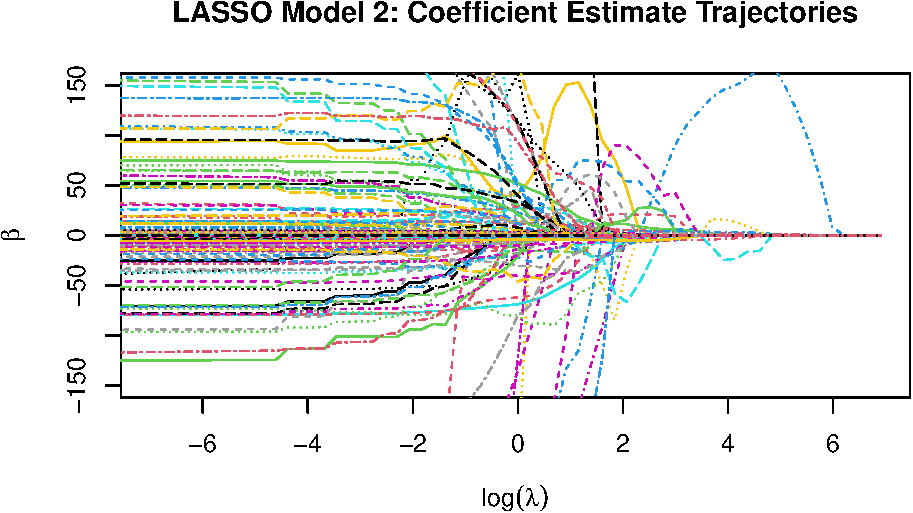
\includegraphics{final_files/figure-latex/unnamed-chunk-34-1.pdf}

In the end, we lean towards accepting the conclusions presented by the
larger second model: With a wider range of interaction effects to
consider, it is less likely that the statistically significant
predictors in this model were only marked as such because they help
explain a relationship between \texttt{cases} and a different predictor
with which they are collinear. Thus, the LASSO models suggest that there
is a statistically significant relationship between \texttt{religious}
and \texttt{cases}, and that the nature of this relationship changes
based on the value of \texttt{mask.mandated.days}. Interestingly, in
LASSO-Selected Model 2, the interaction coefficient
\texttt{religiousYes:mask.mandated.days} has a positive coefficient: An
increase in the number of mask mandated days during the 2020-21 academic
year is associated, in this model, with an increase in the change that
we would expect for a given school if that school were to have a
religious affiliation, compared to if that same school were to not have
a religious affiliation. This phenomenon also seems to be present in
LASSO-Selected Model 1, in which the coefficient estimate for
\texttt{religious:mask.mandated.days} is also positive.

\hypertarget{hierarchical-multi-level-models}{%
\section{Hierarchical Multi-level
Models}\label{hierarchical-multi-level-models}}

We next chose to explore the relationship between 2020 Covid cases and
our list of predictors using hierarchical multi-level models, namely the
mixed effects models from the \texttt{lme4} package in R. We thought
this model type would work well with our data because the data can be
organized hierarchically as follows: The first level is at the
university level; each university has predictors, such as
\texttt{grad.rate} and \texttt{religious}, which are specific to each
university. The second level in the hierarchy is the state level, where
universities in each specific state will share cultural, legislative,
etc. characteristics that can be vaguely accounted for by sorting the
``groups'' by state. For example, mask mandates, which were decided by
state, were in effect at that stage of the pandemic.

A capability of the \texttt{lme4} mixed effects package is that it can
produce both random intercept and random slope models. We decided that
with the data we have, we can only look at random intercept mixed
effects models. This is due to the number of observations we have; there
are a total of 1,705 universities, which means that in each group (by
state + Washington DC), there is an average of just over 33 data points
per group. Especially given the differing densities of universities
(there are 60 in Massachusetts alone), there are simply not enough
observations per group to justify fitting and analyzing a random slope
model. The nature of the random slope mixed effects models means they
will not overfit to the fewer observations in a given group.

First, we fit a model with all of the predictors from our ``base
model'', except \texttt{total.headcount}, which we accounted for using
the ``weights ='' functionality of the \texttt{lmer} modelling. We used
a random intercept model and grouped by state, meaning that the results
include the coefficients for each predictor, which are fixed by state,
as well as the intercept, which should differ by state. Below is a plot
of the coefficient values.

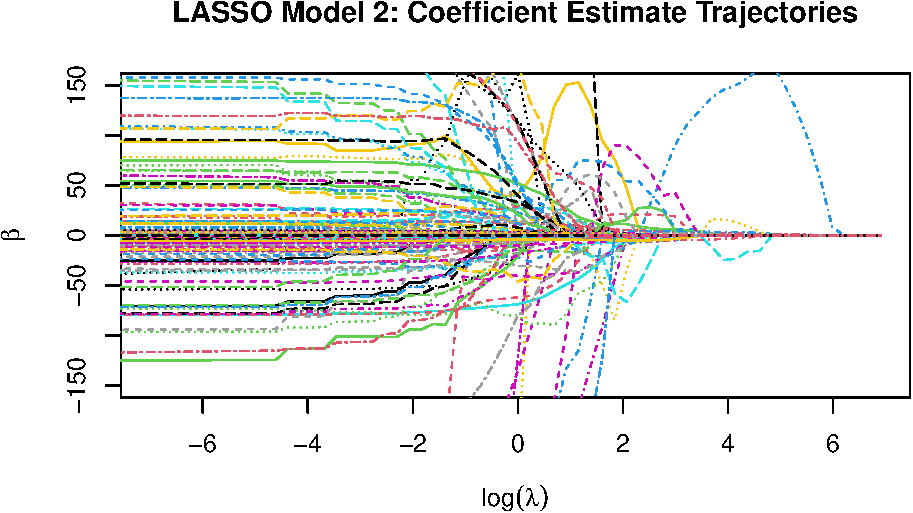
\includegraphics{final_files/figure-latex/unnamed-chunk-35-1.pdf}

We see in the above plot that certain coefficent estimates are
significantly larger than the others. It is worth noting that the
coefficient estimate for \texttt{religiousYes} is actually negative in
this model, which is contrary to all previous models we have explored;
it is not, however, statistically significant, since the confidence
interval covers zero.

To visualize this random intercept model, we created the plot below,
which explores the relationship between \texttt{percent.black} and 2020
Covid cases in institutions; it includes the slopes for each state (and
DC) generated from our mixed effects (random intercept) model. We can
see that the states have some spread in terms of differing intercepts.
We can also see that, similar to the interaction models we explored,
there is no significant visual relationship between religious
institutions (red dots) and non-religious (blue dots) when comparing
\texttt{percent.black} and \texttt{full.cases}. Here, we chose
\texttt{percent.black} for the x-axis, because unlike \texttt{private}
and \texttt{on.campus.housing}, it is a continuous predictor, and unlike
\texttt{percent.pacific.islander} and \texttt{percent.american.native},
it does not have a lot of universities with 0\%.

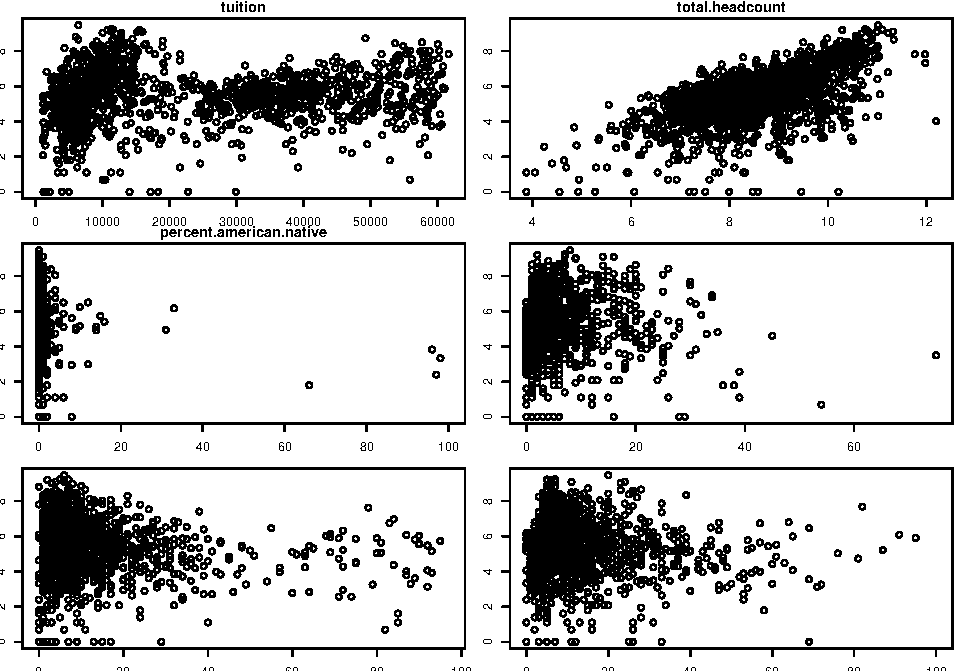
\includegraphics{final_files/figure-latex/unnamed-chunk-36-1.pdf}

Next we explore the relationship between \texttt{gap20repub} and
\texttt{religious} and their interactive effect on 2020 Covid cases
grouped by state (still using mixed effects, random intercept). We use
random intercept models to do so, because of the way in which mixed
effects models allow one to implement predictors at the group (state)
level. \texttt{gap20repub} is unique by state, but does not take on a
unique value in the institutions in each state. We formally test below
whether the effect of university religious affiliation (on 2020 Covid
cases) depends on \texttt{gap20repub}, i.e., whether including the
interaction effect between \texttt{religious} and \texttt{gap20repub}
adds statistically significant explanatory power to the model:

\begin{center}
![](final_files/figure-latex/unnamed-chunk-37-1.pdf)<!-- --> 
\end{center}

The result of the likelihood-ratio test between nested mixed effects
models (one with the interactive effect, one without) indicates that
there is evidence that the interaction between \texttt{gap20repub} and
\texttt{religious} is significant in the predictive model, and the
effect of religious affiliation upon 2020 Covid cases does depend on
\texttt{gap20repub}. Though this was not flagged as a particularly
significant interaction in the above models ---~probably because of
collinearity between \texttt{gap20repub} and other predictors --- it is
not surprising, per se: It is clear that the \texttt{religious}
significantly interacts with many other predictors.

We recreate this analysis for \texttt{mask.mandated.days}, another
predictor that varies at the state level, and again find, via the
likelihood-ratio test, that the mixed-effects model with the interaction
term between \texttt{religious} and \texttt{mask.mandated.days} adds
significant explanatory power to the model:

\begin{center}

```
##   Chi.Sq.Statistic Df    p.value
## 1         6.301377  1 0.01206442
```
\end{center}

Thus, in the context of these hierarchical models, both of these
interaction effects appear to add significant explanatory power to the
model (though not shown, both models above add significant explanatory
power over the random intercept model with \texttt{religious} as the
only predictor).

\hypertarget{sensitivity-analysis-using-poisson-regression}{%
\section{Sensitivity Analysis using Poisson
Regression}\label{sensitivity-analysis-using-poisson-regression}}

In ``Checking the Assumptions of Linear Regression Models'', we found
behavior in our data set that calls into question the assumption of
homoskedasticity that is used in all of the above methods, which are
based on Gaussian regression. Because our response is count data,
Poisson regression is an obvious candidate for improving the violation
of this assumption. The first thing we do to verify this fact is to fit
a Poisson regression model using the same formula as our base model from
above; as the residuals versus fitted values plot below shows, Poisson
regression does, for the most part, fix the intractable violations of
homoskedasticity that we encountered with Gaussian regression.

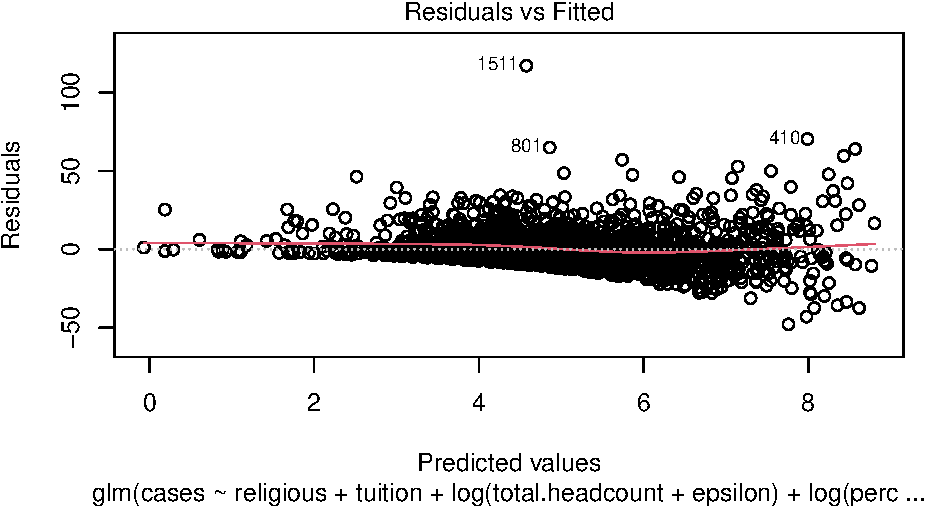
\includegraphics{final_files/figure-latex/unnamed-chunk-39-1.pdf}

With this model, however, the problem is not completely solved: Because
the spread in the responses seems to increase as fitted values increase,
it seems that weighted regression would be the best approach in the
Poisson setting. The most obvious candidate for weights is the predictor
\texttt{total.headcount} --- it is reasonable to think that as school
size increases, the differences approaches to handling the outbreak of
Covid-19 might be manifested in increasingly different case count
numbers. The below plot shows that employing weighted-least-squares
Poisson regression using \texttt{1/total.headcount} as weights for the
most part fixes the problem of heteroskedasticity.

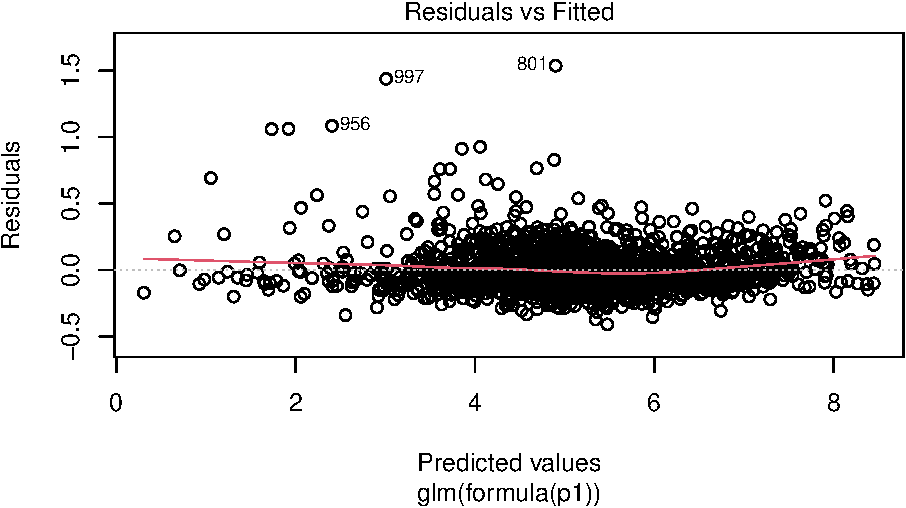
\includegraphics{final_files/figure-latex/unnamed-chunk-40-1.pdf}

Clearly, there are still some outliers, which might be due to a number
of factors, including exceptionally frequent testing, comprehensive
Covid contact tracing systems, superspreader events on campus, or simply
exceptionally large outbreaks on campus; however, the assumption of
homoskedasticity now seems to be reasonable enough to trust our standard
errors.

We now fit Poisson regression models using the same formulas as the most
notable Gaussian models, and compare the lists of coefficient estimates
related to religious affiliation marked as statistically significant by
the two approaches. Note that when determining the statistical
significance of a coefficient estimate in the Poisson models, we use
heteroskedastic-consistent standard errors to account for possible
violations of distribution assumption that the mean of the response is
equal to its variance. The tables below illustrates the results of these
analyses.

\begin{table}

\caption{\label{tab:unnamed-chunk-41}Base Model: Gaussian vs. Poisson}
\centering
\begin{tabular}[t]{l|r|r|r|r}
\hline
coefficient & Gaussian.Estimate & Gaussian.p.value & Poisson.Estimate & Poisson.p.value\\
\hline
gap20repub & 0.0127476 & 0.0000000 & 0.0083467 & 0.0000000\\
\hline
grad.rate & 0.0210106 & 0.0000000 & 0.0170122 & 0.0000000\\
\hline
log(percent.asian + epsilon) & -0.1251276 & 0.0257048 & -0.2202536 & 0.0000565\\
\hline
log(percent.black + epsilon) & 0.1946336 & 0.0000088 & 0.1259964 & 0.0080049\\
\hline
log(percent.pacific.islander + epsilon) & -0.2890057 & 0.0146274 & -0.0738136 & 0.6778458\\
\hline
log(total.headcount + epsilon) & 0.9199545 & 0.0000000 & 0.9386192 & 0.0000000\\
\hline
occupational.degreeYes & -0.1840886 & 0.0173571 & -0.1626333 & 0.0050808\\
\hline
on.campus.housingYes & 0.8225306 & 0.0000000 & 0.7586564 & 0.0000000\\
\hline
percent.student.loan & 0.0053149 & 0.0017920 & 0.0030923 & 0.0721520\\
\hline
percent.two.more.races & -0.0254703 & 0.0262692 & -0.0287106 & 0.0491504\\
\hline
percent.white & 0.0178880 & 0.0000000 & 0.0145168 & 0.0000000\\
\hline
percent.women & -0.0107628 & 0.0000245 & -0.0104932 & 0.0001242\\
\hline
privateYes & -0.6765733 & 0.0000051 & -0.2976105 & 0.0214963\\
\hline
tuition & 0.0000174 & 0.0000161 & 0.0000081 & 0.0270510\\
\hline
\end{tabular}
\end{table}

In the base model, only one coefficient that was statistically
significant in the Gaussian model was no longer statistically
significant in the Poisson model: \texttt{percent.student.loan}.
Otherwise, though the p-values may have changed, the predictors that
were statistically significant in the Gaussian model were statistically
significant in the Poisson model as well.

\begin{table}

\caption{\label{tab:unnamed-chunk-42}Full Interaction  Model: Gaussian vs. Poisson
(Only predictors related to `religious`)}
\centering
\begin{tabular}[t]{l|r|r|r|r}
\hline
coefficient & Gaussian.Estimate & Gaussian.p.value & Poisson.Estimate & Poisson.p.value\\
\hline
religiousYes:log(percent.asian + epsilon) & -0.3936018 & 0.0422889 & -0.2979514 & 0.0457438\\
\hline
religiousYes:log(percent.black + epsilon) & -0.4388041 & 0.0288920 & -0.1931332 & 0.2352499\\
\hline
religiousYes:mask.mandated.days & 0.0017751 & 0.0350710 & 0.0004273 & 0.4971038\\
\hline
religiousYes:on.campus.housingYes & -1.4964379 & 0.0384122 & -1.1822020 & 0.0390593\\
\hline
\end{tabular}
\end{table}

With respect to the \texttt{fullInteraction} model, of the linear or
interaction effects related to the predictor \texttt{religious}, two of
the four coefficient estimates remained statistically significant in the
Poisson model --- \texttt{religiousYes:log(percent.asian\ +\ epsilon)}
and \texttt{religiousYes:on.campus.housingYes} --- while the other two
did not.

\begin{table}

\caption{\label{tab:unnamed-chunk-43}LASSO-Selected Model 2: Gaussian vs. Poisson
(Only predictors related to `religious`)}
\centering
\begin{tabular}[t]{l|r|r|r|r}
\hline
coefficient & Gaussian.Estimate & Gaussian.p.value & Poisson.Estimate & Poisson.p.value\\
\hline
religiousYes & 3.1755840 & 0.0407812 & 2.6427005 & 0.0102538\\
\hline
religiousYes:mask.mandated.days & 0.0016696 & 0.0474806 & 0.0001859 & 0.7572110\\
\hline
\end{tabular}
\end{table}

In the Poisson regression version of LASSO-Selected Model 2, only the
coefficient estimate for \texttt{religiousYes} remained statistically
significant; \texttt{religiousYes:mask.mandated.days} was no longer
statistically significant after we assumed that the errors took on the
Poisson distribution.

\small

\begin{table}

\caption{\label{tab:unnamed-chunk-44}Backwards Sequential Variable Selection Model: Gaussian vs. Poisson
(Only predictors related to `religious`)}
\centering
\begin{tabular}[t]{l|r|r|r|r}
\hline
coefficient & Gaussian.Estimate & Gaussian.p.value & Poisson.Estimate & Poisson.p.value\\
\hline
religiousYes:log(percent.asian + epsilon) & -0.3802799 & 0.0035695 & -0.1859713 & 0.0945386\\
\hline
religiousYes:mask.mandated.days & 0.0020786 & 0.0001400 & 0.0008273 & 0.0473759\\
\hline
religiousYes:on.campus.housingYes & -1.3120944 & 0.0051891 & -1.1023241 & 0.0048741\\
\hline
\end{tabular}
\end{table}
\normalsize

Of the three \texttt{religious} interaction effects that were determined
to be statistically significant in the Gaussian \texttt{back.step}
model, only two remained statistically significant in the Poisson
regression recreation of this model:
\texttt{religiousYes:mask.mandated.days} and
\texttt{religiousYes:on.campus.housingYes}.
\texttt{religiousYes:log(percent.asian\ +\ epsilon)} was not
statistically significant in the Poisson model.

Overall, we have observed that most of the coefficients that were marked
as statistically significant in the Gaussian models fit earlier in the
paper remained statistically significant under the assumptions of
Poisson regression. This corroborates our analyses and findings from
earlier in the paper, and allows us to now draw the overarching
conclusions of our analysis.

\hypertarget{conclusions-and-discussion}{%
\section{Conclusions and Discussion}\label{conclusions-and-discussion}}

Ultimately, we conclude that there is some association between the
religious affiliation of a university and the Covid case counts that it
reported during the fall 2020 semester --- the relationship between
these two variables, however, is nuanced, with interaction effects
between \texttt{religious} and other predictors in our data set playing
a large part. In particular, we found that the interactions between
\texttt{religious} and each of \texttt{mask.mandated.days} and
\texttt{on.campus.housing} to be statistically significant across many
of our models, even in those models constructed using Poisson regression
in our sensitivity analysis.

We found the interaction between \texttt{mask.mandated.days} and
\texttt{religious} to be statistically significant in all but the
forward step model beginning from the intercept, LASSO-Selected Model 2,
and the Poisson regression versions of the \texttt{fullInteraction} and
the second LASSO-Selected linear models. In most models, the coefficient
estimate of this interactive effect was approximately 0.002. This small
but positive value indicates that a religious affiliation is associated
with a greater change in the number of cases that we would expect from a
university if \texttt{mask.mandated.days} were to increase in the state
in which that university is located, compared to a school with the same
predictor set but with no religious affiliation. This indicates that
state-mandated masking initiatives were disproportionately less
effective for religious institutions, which could also be reflective of
the fact that non-religious institutions also include public
universities that may more strictly comply with masking mandates given
their funding ties to state governments.

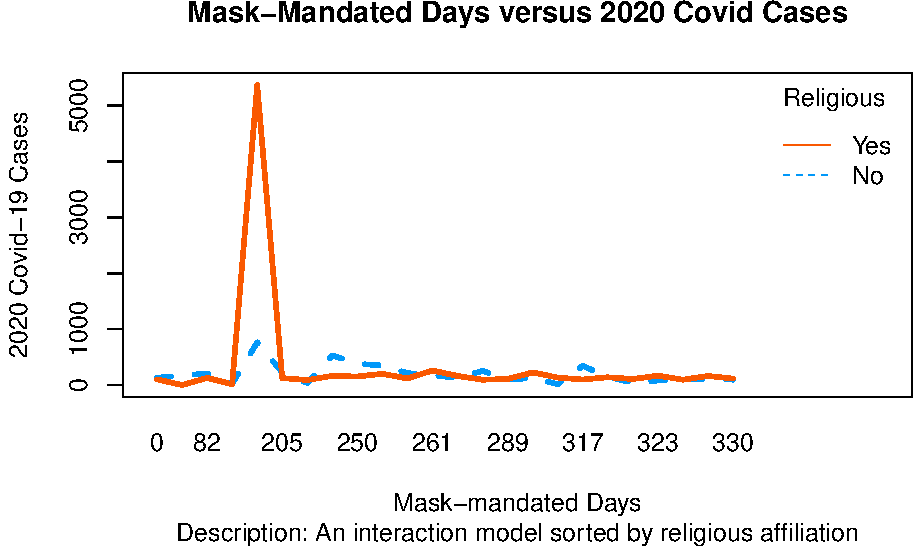
\includegraphics{final_files/figure-latex/unnamed-chunk-45-1.pdf}

The interaction model pictured visually displays some of the
relationship we have found between the interaction
\texttt{religiousYes:mask.mandated.days} and 2020 Covid-19 cases. The
plot peaks just below 205 mask-mandated days, which corresponds to Utah
and/or New Hampshire. We see that in perhaps just a couple of states
with around 175 mask-mandated days, religious institutions have
significantly higher numbers of Covid-19 cases than their non-religious
counterparts. Note that this visual does not take into account
confounding variables, whereas the models we discussed do.

Likewise, the interaction between \texttt{on.campus.housing} and
\texttt{religious} was statistically significant in all but the forward
step model beginning from the intercept, LASSO-Selected Model 2, and the
Poisson regression version of the latter. Across all models, the
coefficient estimates for this interactive effect ranged from about
-1.71 to about -1.28; interestingly, this can be interpreted as an
indication that a religious affiliation decreases the expected change in
cases that we would expect if a given school were to offer on campus
housing, compared to if that school were to not offer on campus housing
to its students.

With such strong evidence in favor of the statistical significance of
both of these interactive effects, we are inclined to conclude that
these interactive effects are indeed important. But is simply having a
religious affiliation alone associated with changes in fall 2020 Covid
case counts? We did not reach a clear conclusion with our analysis ---
there was disagreement between the models we considered in terms of the
statistical significance of the linear effect of the \texttt{religious}
predictor. While this predictor was statistically significant in the
\texttt{religiousInteraction} model, LASSO-Selected Linear Model 2, and
the Poisson regression version of the latter, it was not statistically
significant in the base model, the \texttt{fullInteraction} model, the
any of the sequential variable selection models, our hierarchical model,
or the Poisson regression versions of any of these models. Overall,
because of this disagreement, and because the majority of models
actually did not find the \texttt{religious} predictor to be
statistically significant, we do not conclude that there is an
association between whether a university has a religious affiliation and
its reported fall 2020 Covid case counts. Rather, the relationship found
between the religious affiliation of a university and its 2020 Covid-19
cases in certain models can likely be attributed to confounding social
effects, and models that did not find a statistically significant
relationship accounted for these confounding variables and interactions.

One of the most surprising results of our analysis was the absence of
\texttt{gap20repub} from our statistically significant results. Because
the Covid-19 pandemic was such a politicized issue, we expected this
predictor --- which was a stand-in for the differences in Covid-19
policies between blue and red states --- to play a large role in our
analysis with respect to religious affiliation. In reality, it never
seemed to come up as important. Indeed, the only time that the
interaction effect between \texttt{religious} and \texttt{gap20repub}
was statistically significant was when we specifically isolated these
two predictors in one of our simple random intercept models; otherwise,
this interaction effect never played a major part. \texttt{gap20repub}
itself ---~as well as interactions with predictors other than
\texttt{religious} ---~was also not found to be statistically
significant in many of our models. It is possible that our predictor
\texttt{mask.mandated.days} captured enough information about the
responses to the Covid-19 pandemic in each state to properly inform our
models. This is not to say, however, that this predictor was entirely
useless in this analysis --- it was the only way that we were able to
capture potential intangible confounding political variables that would
have been difficult to capture quantitatively, such as prevailing
attitudes as to the severity of the pandemic in a given state. In the
end, though \texttt{gap20repub} did not play a very important part in
the interaction effects explored in this paper, we believe that the
association between political attitudes or voting behaviors and Covid-19
case counts --- at universities or at large --- deserves its own
dedicated exploration.

\end{document}
